\documentclass[onecolumn, a4paper,11pt, headings=small, titlepage=true]{scrartcl}
\usepackage[utf8]{inputenc}
\usepackage{amsmath,amssymb,amsfonts}
\usepackage[english]{babel}
\usepackage{url}
\usepackage{hyperref}
\usepackage[left=1.7cm, right=1.7cm, top=2cm, bottom=2.3cm]{geometry}

\usepackage{enumitem}
\setlist[description]{leftmargin=\parindent}%, noitemsep

% Remove page number from titlepage
\renewcommand*{\titlepagestyle}{empty}

\RedeclareSectionCommands[
  beforeskip=.5\baselineskip,
  afterskip=.3\baselineskip
]{section, subsection, subsubsection}

\begin{document}
\author{Cay Rahn - 6255648}
\date{\today}
\title{Investigating the molecular cause of hypermobile Ehlers-Danlos syndrome}
\subtitle{MSB 1014 - Network Biology}

\maketitle

\clearpage
\pagenumbering{arabic}
\setcounter{page}{1}

% 2-3 pages without title page, figures, tables and references
% max 5 figures/tables - every figure/table has a caption title and descrption

\section{Introduction}

% Funnel shape (start broad, become more specific, leading to the research question)
% General description of the background and gaps that will be filled by the research
% Clear research question

Ehlers-Danlos syndromes are a group of heritable connective tissue disorders that can be classified into multiple subtypes. The current classification describes 14 subtypes \cite{classification2017, Malfait2020}, with hypermobile EDS (hEDS) being the most common form. It is also the only subtype with an unknown molecular cause, leading to a diagnosis based on clinical presentation. Identifying the molecular cause is crucial to improving the diagnosis process, understanding the disease and finding potential treatment options \cite{Ritelli2020}.

Although many studies investigated several genes, no clear molecular cause with a connection to connective tissue has been established yet \cite{Caliogna2021}. While an ongoing study aims to find the genetic cause of hEDS by analysing the genes of around 1000 affected individuals, results are not expected before 2025 \cite{HEDGE}. Until then, utilising already collected data is essential to understand more about hEDS. One problem with this is that the diagnosis criteria changed in 2017, resulting in data from before the change not being usable anymore \cite{Gensemer2021, Ritelli2022}.
%
%
%\begin{itemize}
%	\item we know the clinical representation and how other eds types work (kind of)
%	\item TODO: include information of what is affected, extracellular matrix, collagen, connective tissue
%\end{itemize}

This project aims to investigate the molecular cause of hypermobile EDS by studying the influence of differentially expressed genes in hEDS patients. It mainly tries to find molecular functions and biological processes affected by differentially expressed genes that are similar to the ones affected by the molecular cause of other EDS types. This analysis eventually aims to find genes differentially expressed in hEDS that are candidates for being the molecular cause of hEDS and to relate the findings to existing research.
\section{Methods}
% Structure with subsections
% Methodology aligns with research question (appropriate resources/methods used)
% General description of the methodology
% Enough details to ensure the reproducibility of results
The following structured approach will be pursued to answer the research question:

\begin{description}[leftmargin=5pt]
	\item [Analysis of Differentially Expressed Genes (DEGs).]\label{sec:methods-deg}The used dataset of gene expression profiles from dermal fibroblasts from patients with hEDS and healthy controls is available at the NCBI GEO database with the accession number GSE218012 \cite{Ritelli2020}. The analysis is performed with the R-packages DeSeq2 and limma based on the R-Script from GEO2R to identify up-regulated and down-regulated genes \cite{DESeq2, limma}. Genes with a log2-fold change $> \pm 0.5$ and a by the Benjamin-Hochberg procedure adjusted p-value $< 0.05$ are included. The cut-offs were chosen based on similar research \cite{Karimizadeh2019, Lim2019}.

	\item[Network Creation.] The Protein-protein interaction (PPI) network is created in Cytoscape \cite{Cytoscape} by querying the before-identified DEGs from the STRING database with an interaction score $> 0.4$, which reflects medium confidence \cite{StringDB}. Since hEDS belongs to the family of Ehlers-Danlos syndromes, its molecular cause is most likely closely related to other EDS types. The PPI network of the DEGs is therefore expanded by additionally querying genes related to other EDS types retrieved from Disease ontology (Disease Ontology ID 13359) \cite{DO}. The resulting network is annotated with the differential expression data.
	
	\item[Gene Ontology and Clustering.]GeneOntology (GO) enrichment is performed using the R-package clusterProfiler to gain insight into biological processes and molecular functions affected by DEGs, with results with $p < 0.05$ being considered significant \cite{Ashburner2000,Consortium2023, Wu2021}. To attain more detailed insights into specific parts, the created network is clustered using two different algorithms, resulting in different cluster structures: MCODE to analyse the molecular function and Community clustering to investigate biological processes. Only clusters of more than 15 genes are considered to ensure relevance and keep the analysis feasible. Further analysis of the resulting clusters includes investigating whether genes are clustered with genes that cause other EDS types and whether the clusters consist of up-regulated or down-regulated genes or a combination of both.
	
	\begin{description}[leftmargin=0pt]
		\item[MCODE]MCODE is a clustering algorithm designed to find highly connected regions in PPI networks that might represent molecular complexes \cite{mcode}. MCODE was applied in Cytoscape with the clusterMaker2 app using the default parameters \cite{Cytoscape, clusterMaker2}.
		
		\item[Community Clustering]GLay, a community clustering algorithm, was designed to be used for a functional interpretation of clusters in networks and used for this purpose here \cite{GLay}. Analogous to the MCODE, clustering was performed with clusterMaker2 and Cytoscape using the default parameters \cite{Cytoscape, clusterMaker2}.
		
		Heat Diffusion is applied on larger clusters to identify genes closely connected to EDS genes that are not captured by smaller clusters, starting with the EDS nodes using Cytoscape functionality \cite{heatDiffusion}, using a time parameter of $t=0.3$.
	\end{description}
\end{description}


%[TODO: position of eds genes in network - why]
\section{Results and Discussion}
% Structure with subsections
% Use of figures/tables (max. 5)
% General description of the results
\subsection{Differentially Expressed Genes and Network Creation}

Under the chosen thresholds discussed in section \ref{sec:methods-deg}, 908 genes were found to be differentially expressed. Around half (495) are up-regulated, and the remaining 413 are down-regulated. STRING could query 828 of them; using other ID types did not change this. After querying the additional EDS-related genes, the resulting network consists of 847 genes and 6129 connections.

The position of the known EDS genes in the network is, on average, more central than expected by chance based on degree, clustering coefficient, betweenness centrality and closeness centrality, supporting the close relationship between hEDS and other EDS types.

\subsection{Enrichment analysis and clustering}

GO-enrichment is performed on the DEGs to acquire an overview of over-represented molecular functions, biological processes and cellular components. In contrast to later results, which include the known EDS genes, this analysis is performed purely on the differentially expressed genes.

Biological processes over-represented in the DEGs include cell-cycle regulation, signalling and transition, nucleosome assembly and organisation and protein-DNA assembly and organisation.  Cellular components affected are the nucleosome (GO:0000786), the chromosomal region (GO:0098687 and GO:0000775), the protein-DNA complex (GO:0032993) and the collagen-containing extracellular matrix (ECM) (GO:0062023). Over-representation analysis for the molecular function is less meaningfull on a large network. Still, three terms are related to a significantly higher number of genes than the rest: The structural constituent of chromatin (GO:0030527), protein heterodimerization activity (GO:0046982) and extracellular matrix structural constituent (GO:0005201).

[TODO: Do i want to look at Pathways? lupus and alcoholism maybe not that interesting, but Cell cycle?]

[TODO: Analysis]

\subsubsection{MCODE}
Running MCODE on the created networks finds 3 clusters with more than 15 genes, one with 66 genes and 1953 connections, one with 44 genes and 686 connections and one with 16 genes and 114 connections, with the two larger clusters containing up-regulated genes only and no genes known to cause other EDS types. % TODO: interpretation - might those be processes that we see only in hEDS and not in other EDS types? Look at heat in community cluster

\paragraph{MCODE cluster with EDS genes}
The third, smaller cluster, shown in Figure \ref{fig:mcode3}, contains mainly up-regulated but also two down-regulated genes. Some do not show a high differential expression but are genes known to cause other EDS types. The cluster consists of eight EDS genes with a $|\text{log2FoldChange}| < 0.5$ and nine differentially expressed genes. One of the EDS genes is also one of the two down-regulated genes. All known EDS genes besides ADAMTS2 have a high Closeness Centrality, consistent with the findings of EDS genes being more central in the complete network. COL21A1 shows the highest differential expression ($\text{log2FoldChange} > 2$), more than twice as high as the other genes while being less central in the cluster.

\begin{figure}[htb!]
	\centering
	\caption*{\textbf{MCODE cluster with EDS genes}}
	\begin{subfigure}{.49\textwidth}
		\centering
 		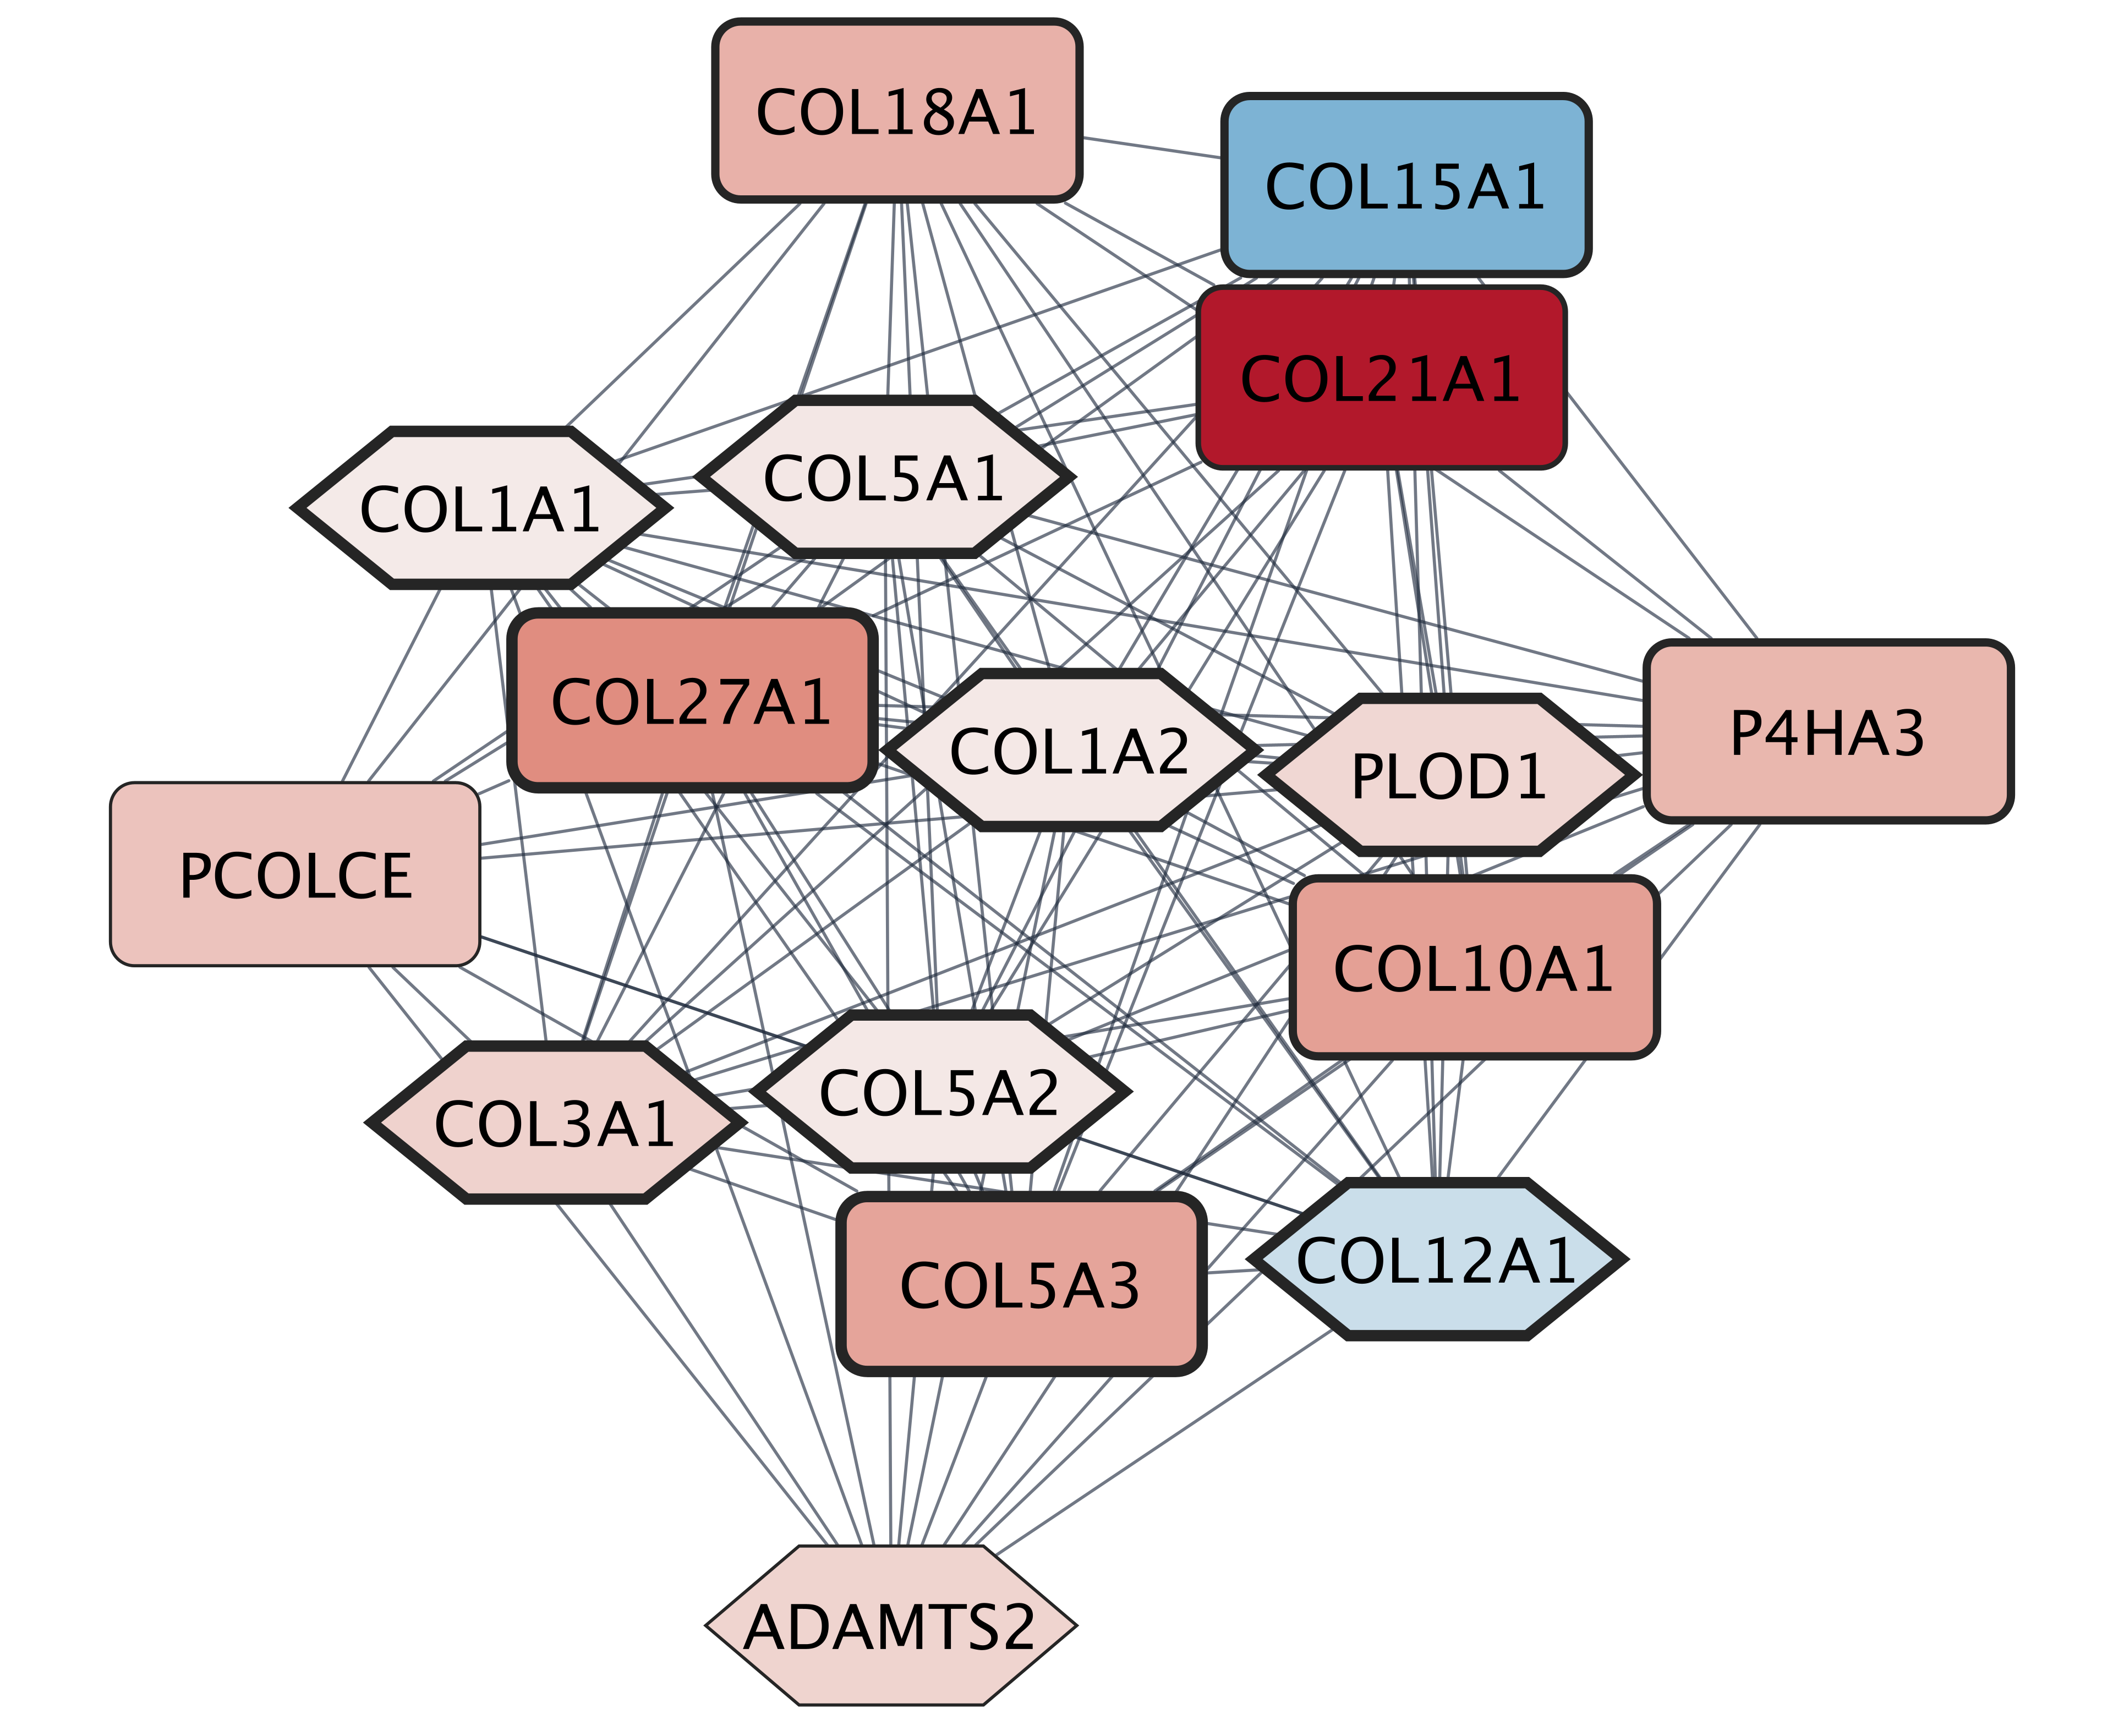
\includegraphics[width=\textwidth]{fig/mcode-cluster-without-enrichment.png}
 			\caption{Without visualization of the ECM GO term}
 	\end{subfigure}
 	\begin{subfigure}{.49\textwidth}
 		\centering
 		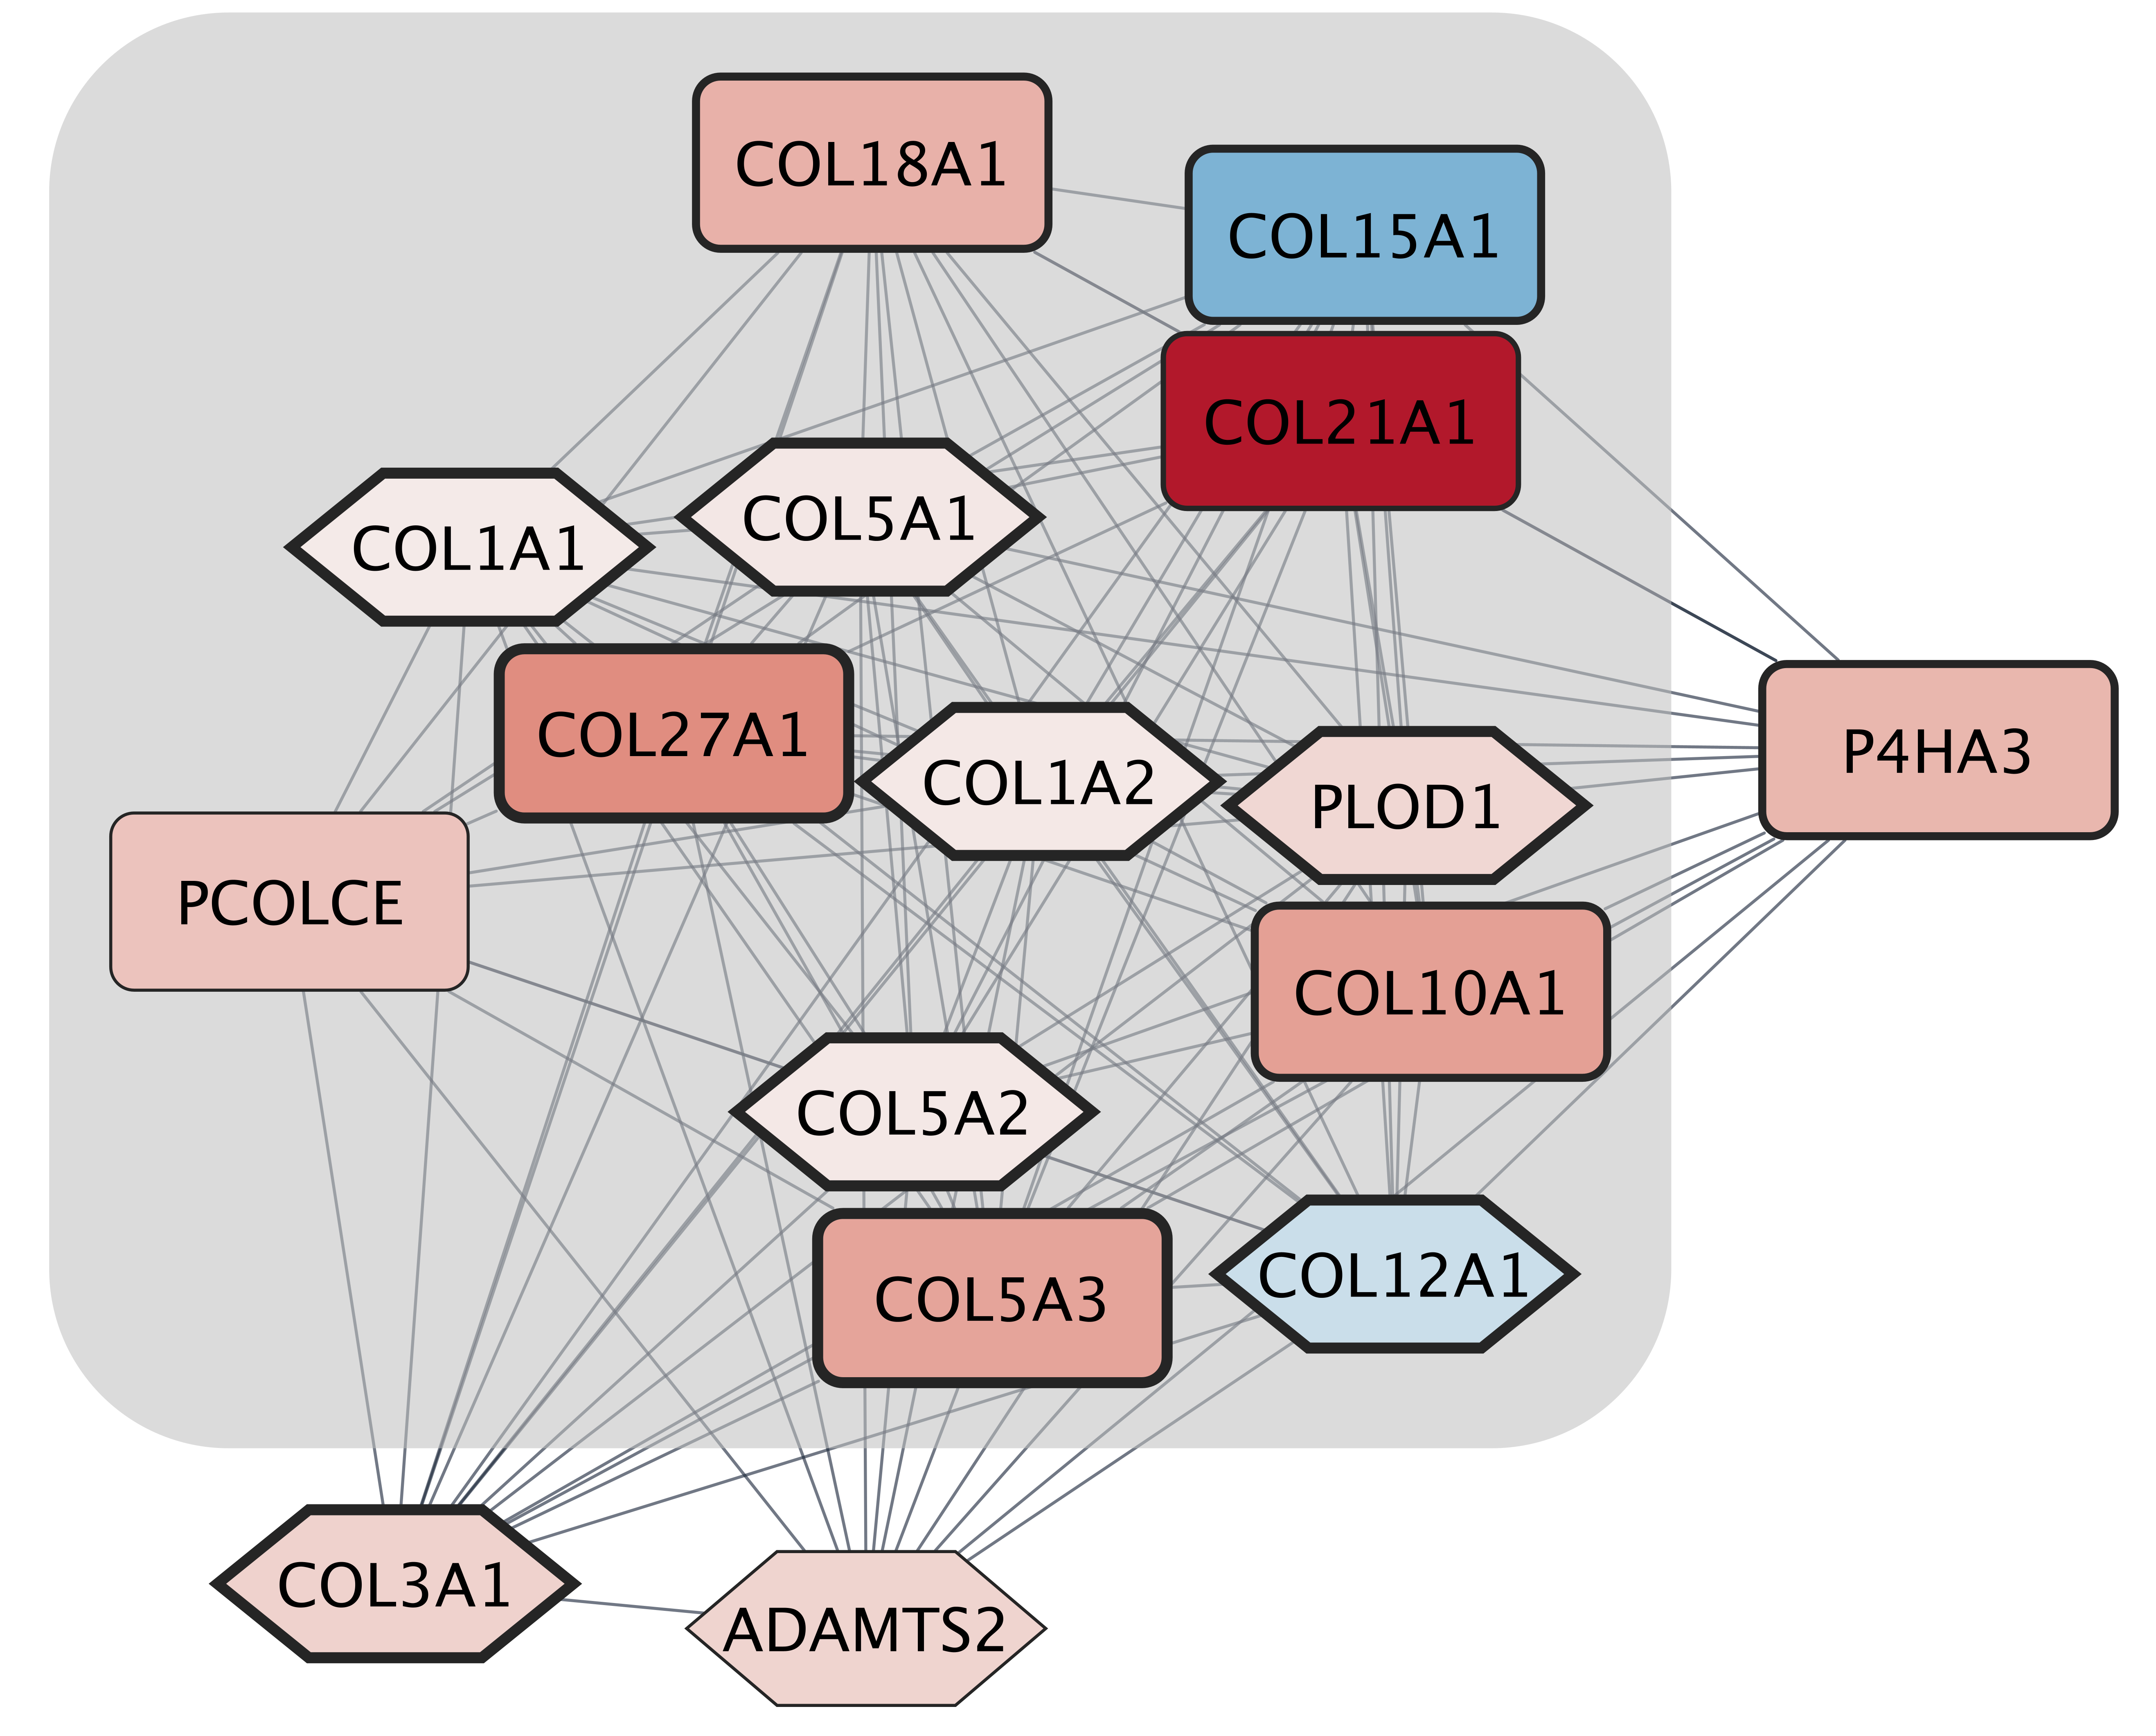
\includegraphics[width=\textwidth]{fig/mcode-cluster-eds-genes-with-ecm.png}
 		\caption{With visualization of the ECM GO term}
 	\end{subfigure}
	\caption[MCODE cluster with EDS genes]{\centering The MCODE cluster contains many genes known to cause other types of EDS. [TODO: add legend for shape, border and colour]}
	\label{fig:mcode3}
\end{figure}

GO-Enrichment testing overrepresentation of molecular functions of the cluster returns extracellular matrix in two terms, GO:0005201 and GO:0030020, with the second one being a subterm of the first. The first describes the action of a molecule that contributes to the structural integrity of the extracellular matrix; the second is a constituent of the extracellular matrix that enables the matrix to resist longitudinal stress. Both GO terms contain the same EDS genes and seven, respectively, six other genes, with PCOLE being the only gene not present in the GO subterm. These genes are investigated in more detail regarding their centrality, differential expression and what is known about them. COL27A1, a fibrillar collagen gene, has a central position in the cluster and relatively strong differential expression. The same applies to COL5A3, another gene related to collagen. The gene COL21A1 is very strongly differentially expressed, as mentioned before. It encodes the alpha chain of XXI collagen, which maintains the integrity of ECM and is a paralog to COL5A1, a known EDS gene \cite{COL21A1}.

To find connections to ECM in the enrichment analysis is consistent with findings of similar research \cite{Ritelli2022}. [Todo: there was other research, find] The affection of ECM with particular disorganisation of collagen and fibronecting was found in hEDS and two other EDS types \cite{Chiarelli2018}. [TODO: point out what my new findings are, COL21A1, etc.]

\paragraph{Up-regulated MCODE cluster}

The two larger, up-regulated MCODE clusters show no over-representation in ECM terms, as is shown in Figure \ref{fig:mcode-cluster-mf}. It is noticeable that the enrichment of the first cluster shows that only a few genes are part of the enriched terms. For the second cluster, the gene ratio is much higher, with up to around 80\,\% of the genes being involved in the second two terms. Therefore, the enrichment of the first cluster provides little insight into molecular function in hEDS patients.

 \begin{figure}[htb]
 	\centering
 	\caption*{\textbf{Molecular function enrichment for the two larger up-regulated clusters}}
		\begin{subfigure}{.49\textwidth}
			\centering
 			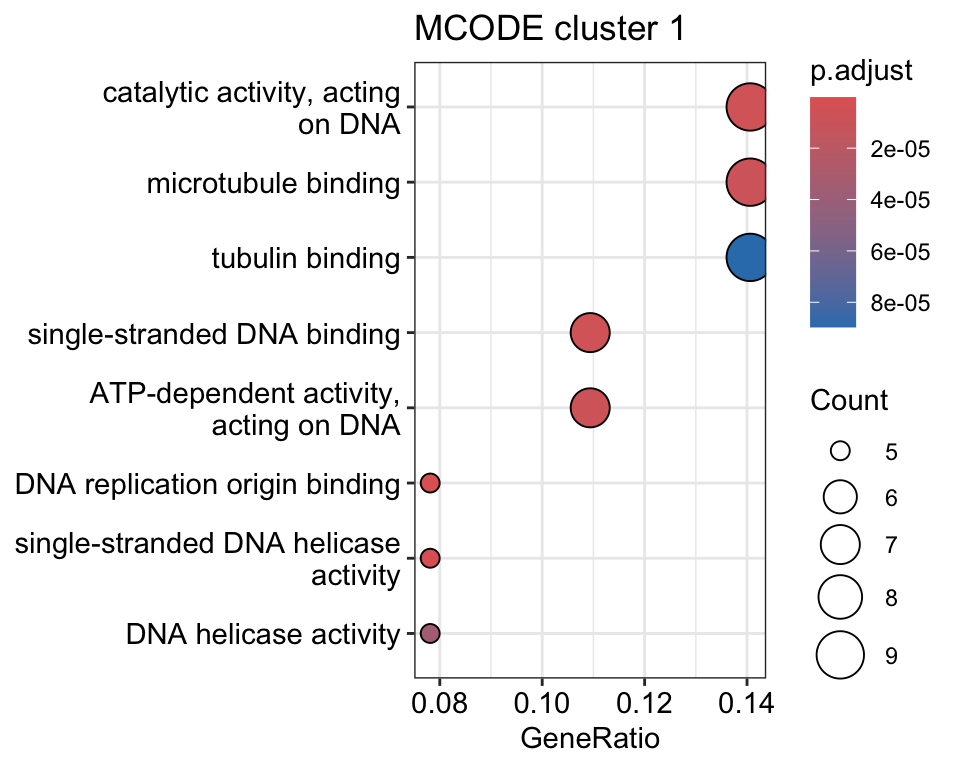
\includegraphics[width=\textwidth]{fig/mf-mcode-cluster1}
 			\caption{First MCODE cluster}
 		\end{subfigure}
    	\begin{subfigure}{.49\textwidth}
    		\centering
 			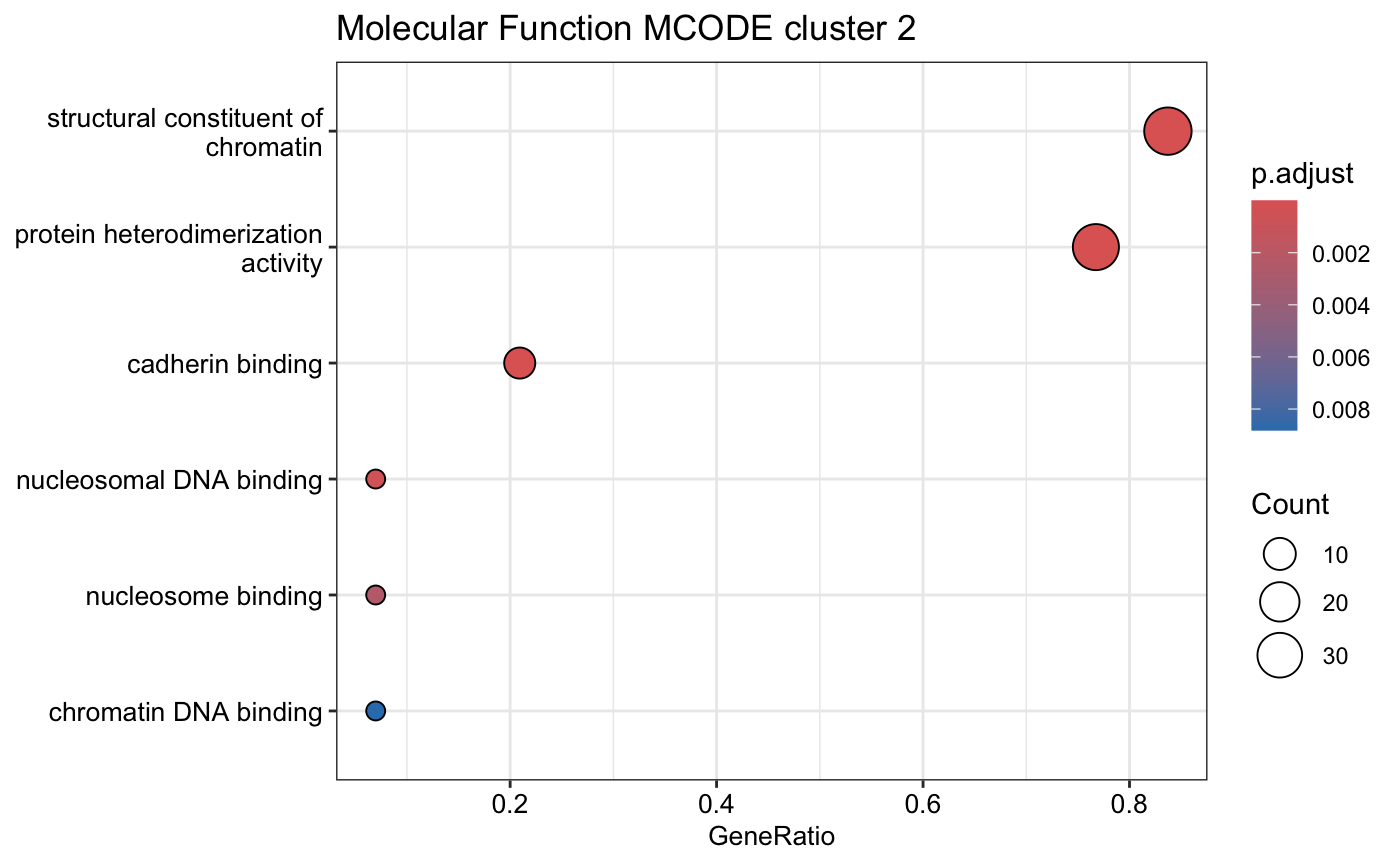
\includegraphics[width=\textwidth]{fig/mf-mcode-cluster2.png}
 			\caption{Second MCODE cluster}
 		\end{subfigure}
 	\caption{The results of the GO-enrichment for molecular function of the two up-regulated, larger MCODE clusters}
 	\label{fig:mcode-cluster-mf}
 \end{figure}

On the other hand, the up-regulation seen in the second cluster for the GO-term GO:0030527, the structural constituent of chromatin, is interesting because earlier research found down-regulated genes involved in processes related to chromatin in vEDS \cite{Chiarelli2018}.


\subsubsection{Community Clustering}

Community Clustering results in six clusters with more than 15 genes. Three are very small and loosely connected clusters, containing 18 to 29 genes and approximately the same amount of connections as genes. Since clusters of less than 20 genes are not large enough for analysis of biological processes, smaller clusters are omitted from the analysis. Additionally, there are two medium-sized highly connected clusters with 76 genes and 100 connections, and 105 genes and 2330 connections, respectively, and one huge cluster with 363 genes and 1661 connections.

\paragraph{Medium Sized Community Clusters}

The medium-sized clusters are highly interconnected and contain mainly up-regulated genes. Genes related to Nucleosome and protein-DNA complex are part of one of the clusters while the genes related to the chromosomal region are clustered in the other one.
\begin{itemize}
	\item first one: 5 highly differentielly expressed genes noticeable: H3C2, H3C7, H2BC10, ASF1B, WDR37
\end{itemize}


\paragraph{Largest Community Cluster}

The largest cluster contains a mix of up-regulated and down-regulated genes, and all 21 genes related to other EDS types. Furthermore, it contains all  genes being part of the GO-term for the ECM found in the over-representation of molecular functions of the MCODE cluster containing the EDS genes. The molecular cluster showing enrichment towards the chromatin part is not a part of this community cluster.

Heat Diffusion starting at EDS genes finds 39 DEG with a heat $> 0.1$ beside the starting nodes. These hot genes intersect with the MCODE cluster containing the EDS genes as it is expected due to their close connection reflected in the clustering. Beside those, there are 31 hot genes.

% CLEC3B, LAMA5, MAN1B1, PLS3, TNC (identified in paper), ADAMTS4, LAMB3, LAMB1, SLC4A11, MYLK, MKX, OGN, LOXL4, ASPN, MYH11, OLFML2B, COMP, C4B, HS6ST1 (identified in paper), FNDC1, INHBA, CHPF, LOXL1, GPC4, NUDCD1, ADAMTSL4, CSPG4, SULF1, NETO2 (identified in paper), CNIH3, ITGBL1

[TODO: check whether they were mentioned in other research and if we see them somewhere else]

\subsection{Discussion and Conclusion}

\begin{itemize}
	\item ECM/collagen in genes closely related to genes of other EDS types, seen in community cluster and MCODE cluster
	\item TODO: link to research, meaning
	\item chromatin related terms in a MCODE cluster and a community cluster found, in community cluster together with nucleosome
	\item chromatin interesting because down-regulated in other EDS type
	\item TODO: link to research, meaning
	\item heat diffusion in largest community cluster showed other genes additionally to ECM genes that are probably interesting
	\item project showed genes fullfilling similar roles than genes in other EDS types, candidates for causing hEDS
	\item hEDS has wide spectrum of representations, probably multiple components represented in the found clusters
\end{itemize}

% all chromatin genes in Community cluster 5
\chapter{Discussion}
% Structure and coherence in discussion
% Discussion of the (expected and unexpected) results and link to existing literature
% Conclusion / refers back to research question

\bibliographystyle{vancouver.bst}
% Quality of literature used (biological background / methodology / tools)
% Number of references (>20)
% References style (Vancouver)
\bibliography{references.bib}
\end{document}